\documentclass[12pt,journal,compsoc]{IEEEtran}
\providecommand{\PSforPDF}[1]{#1}
\hyphenation{op-tical net-works semi-conduc-tor}
\usepackage{graphicx}
\usepackage{float}
\floatstyle{boxed}
\restylefloat{figure}

\begin{document}
\title{Evolutionary Design of Particles for Collectively Intelligent Problem Solving}
\author{Benjamin~Bengfort,~Kevin~Harrison,~and~Philip~Kim}

% make the title area
\maketitle

\begin{abstract}

Emergent, self-organizing flocks of particles can be implemented using only simple, local movement behavior rules. When particles are also improved with a limited working memory and goals, the local interactions of these top-down controllers leads to emergent global problem solving such as search and retrieve. We will show in this paper that the rules for both movement and goals can be evolved using Evolutionary Computing techiques on the dynamics parameters, as well as on the finite state machines that control behavior. The evolved particles perform as well as or better then those designed by humans.

\end{abstract}

\section{Introduction}

Ever since Reynolds demonstrated that flocks of birds could be simulated as multi-agent systems \cite{reynolds1987flocks}, there has been interest in improving flocks, schools, and swarms to higher levels of collective intelligence. The relatively simple nature of each agent; its motion or goals are determined solely by local interactions; leads to emergent global behavior. Decentralized control would mean optimal and economic solutions to problems in both algorithmic and physical domains. Furthermore, there has been interest in extending such systems to solve more general problems than traditional optimization \cite{kennedy1995particle}, modeling complex systems \cite{ottino2003complex,clerc2002particle} or cultural algorithms \cite{chung1996testbed}.

This extension has primarily focused on the physical domain to improve multirobot team movement control as in \cite{balch1998behavior,ccelikkanat2010steering,hodgins1994robot}, however higher order problem solving is currently being explored. One large area of research is the deployment of mobile robots or sensors for area coverage, either to map terrain, or to establish mesh communication links. In \cite{cheng2009distributed}, flocking behavior was used to maximize coverage, while still maintaining collective behavior. Other tasks being explored include urban pursuit \cite{winder2004using} and robot herding of animals \cite{vaughan1998robot}.

Many approaches have improved the simple local dynamics by adding minimal, cost effective top down components that also behave locally to produce emergent behavior. One very successful addition to flocks for problem solving is the addition of working memory \cite{winder2012role,hu2003particle}. Building on flocks with memory improvements, Rodriguez in \cite{rodriguez2004extending} added goal-driven intelligence in the form of a finite state machine (FSM) that switched the agent between different sets of movement behaviors according to its local environment and current goal. He was able to demonstrate that a team of such agents was able to solve a resource locate-and-collect problem, and that a team programmed with flocking behaviors outperformed teams of agents that did not influence each other's movements.

These exciting results seem to indicate that in the future difficult environments might be economically explored or exploited by flocking robotic teams exhibiting local behavior for collective intelligence. For example in disaster areas such as fires or earthquakes, teams of flocking robots may be able to more effectively search and rescue victims. Landscapes such as other planetary bodies, the deep sea, or volcanos may similarly be accessible by such teams. However, in order to work in varied terrains and tasks specific swarm systems must be developed by humans to design both the bottom up movement behaviors and the top down controllers. Such design tasks have even led to formal design theory such as \cite{mataric1993designing,capera2003amas}. Although this theory might be applicable to a wide array of problems, a more flexibile approach could enable even more adaptive systems.

Familiar evolutionary computation techniques such as Genetic Programming (GP) \cite{koza1992genetic}, Evolutionary Strategies \cite{rechenberg1989evolution}, and Genetic Algorithms \cite{goldberg1988genetic} have already shown proof of the potential of computational design techniques for machine learning, optimization, and even engineering. Finite state machines have already undergone evolutionary processes to produce better results for particular tasks like automatic target detection \cite{benson2000evolving}. Evolving movement behaviors would be the equivalent of other real value optimization problems. Using these techniques it seems that evolving the individual particles in a swarm would be an effective technique of natural design and adaptation that mimics nature.

This is not to be confused with evolutionary technqiues that leverage swarms as in \cite{wei2002swarm,miranda2005evolutionary}. In this paper, we have attempted to extend Rodriguez's findings in \cite{rodriguez2004extending} by applying evolutionary techniques specifically to the agent control mechanisms. Rodriguez determined the structure of the FSM and the parameters defining each state through inspection and empirical techniques. We attempt to determine the optimal parameters by an evolutionary process that runs a population of randomly-generated FSM configurations through a simulated problem and then evolves the population through fitness-based selection, recombination, and mutation genetic operators.

We will show that a novel finite state machine for movement control can be evolved using an evolutionary programming technique that performs as well as or better that those configured by a top-down design approach. We will present both the simulation using the best human designed parameters, then an evolutionary computation to evolve the individual particles in the simulation.

\section{Methodology}

In order to best demonstrate that an evolutionary process can generate an agent controller that is competitive with a human designed one, we have created an experimental setup that is intentionally similar to the work done in \cite{rodriguez2004extending}. The task is for a team of simulated agents to search and gather resources that are spread across a large two-dimensional world with periodic boundary conditions, then return the resources to a designated home base.

The individuals of the team operate as a flock- local rules determining movement and goals lead to emergent flocking behavior. Each individual has a limited sight range and angle, the ability to communicate with other, nearby agents and a limited working memory. Particle behavior is governed by a finite state machine that determines how each particle moves given its individual state and the environment around it.

The task is competitive, as there are two teams in the environment competing for the resources and therefore the simulation is non-deterministic. Agents can mine resources not only from designated depots, but also steal from the home base of the other team. The winner of a simulation is determined as the team that has the most resources in their home base at the end of a predetermined number of time steps.

The evolutionary process uses this simulation to pit individuals created via genetic operations against the best designed human agent. The fitness of the evolved team is a function of the resources that they have collected vs. the resources the other team collected against them. The next generation of evolution is then dependent of the fitness of teams as run in the simulation. In the parlance of evolutionary computing, the genotype is the real valued vector that represents the finite state machine of the particle and the phenotype is the emergent behavior of the team as a whole as it participates in the simulation.

In this section we will present the details of the simulation, as well as the details of the evolutionary computation mechanism that searches for the optimal, most economic particle in the simulation.

\subsection{Simulation}

The movement behavior of particles in teams is governed by local interactions of particles within a particlar neighborhood. The particle updates its velocity at each timestep based on what it obeserves in the world around it. As a whole, this leads to self-organizing, emergent behavior of the flock as a combined whole of its individuals. In particular, movement behaviors are updated with six velocity components: cohesion, alignment, separation, seeking, clearance, and avoidance. Together these components enable flocking behavior, minimize collisions, and strike a balance between the exploration of the world and the exploitation of discovered minerals.

%TODO: Discuss maximum velocity and other simulation parameters
%TODO: Discuss how the velocity is computed given the velocity components
%TODO: Dicsuss the finite state machine and how it is composed of behaviors

It is important to discuss each individual velocity component in detail, as these components are part of the evolutionary mechanism that we have employed. Every component has several parameters: the radius - the site distance and alpha, the site angle which determine the neighborhood of the particular component. Additionally the weight and priority of the component are used to compute the final velocity of the particle.

Cohesion: a vector pointing towards the average position of friendly agents in the neighborhood, with magnitude equal to zero when the agent's distance to the average neighbor is zero and increasing quadratically with distance until it is equal to the maximum velocity when the distance to the average neighbor is r. The neighborhood includes all team members who are not guarding or stunned.

\[ \vec { v_{ c } } =v_{ max }\frac { \Delta  \vec { p }  }{ \left\|   \Delta \vec { p }  \right\|  } \left( \frac { \left\|  \Delta \vec {  p }  \right\|  }{ r }  \right) ^{ 2 } \]

Alignment: a vector pointing in the same direction as the average velocity of friendly agents in the neighborhood, with magnitude equal to zero when the agent's distance to the neighbors' average position is zero and increasing quadratically with distance until it is equal to the maximum velocity when the distance to the average neighbor is r. The neighborhood includes all team members if they are seeking or spreading.

\[ \vec { v_{ al } } =v_{ max }{\left( \frac { \left\| \Delta \vec { p } \right\|  }{ r }  \right)}^2\frac {\Delta \vec{v}} { \left\| \Delta \vec{v} \right\| } \]

Separation: a vector pointing away from the average position of friendly agents in the neighborhood, with magnitude equal to the maximum velocity when the distance between the agent and the average position is zero, and decreasing quadratically with distance until it is zero when the distance to the average neighbor is r. The nighborhood includes all team members no matter their state.

\[ \vec { v_{ d } } =-v_{ max }\frac {\Delta \vec{p}} { \left\| \Delta \vec{p} \right\| }{\left( \frac { r - \left\| \Delta \vec { p } \right\|  }{ r }  \right)}^2 \]

Seeking, Homing, and Mineral Cohesion: vectors pointing directly towards the target site with a magnitude proportional to the maximum velocity. These velocity components allow the particle to navigate ina  meaningful manner. The target is stored in memory and this velocity component isn't influenced by nearby neighbors.

\[ \vec{v_h} = v_{max} \frac {\vec{p_t} - \vec p} { \left\| \vec{p_t} - \vec p \right\| } \]

Clearance: a vector pointing in a direction orthogonal to the difference between the average neighbor position and the agent's position proportional the the maximum velocity. This component ensures that swarms have a wide field of view. The neighborhood of this component is team members in sight that are not guarding or stunned.

\[ \vec{v_{cl}} = v_{max} \frac {\Delta \vec p_\perp } { \left\| \Delta \vec p_\perp  \right\| }  \]

Avoidance: a vector pointing away from an enemy agent in the neighborhood, with magnitude Vmax when distance to the enemy is zero and decreasing linearly with distance until it is zero when the distance is r. Unlike all the other components, this can be applied multiple times each timestep--once for every enemy in the neighborhood.

\[ \vec { v_{ av } } =\sum _{i=0}^{n} {v_{ max } \left( \frac{r - \left\| \Delta \vec{p_e} \right\|} {r} \right) \frac { \Delta \vec { p_e }  }{ \left\| \Delta \vec { p_e }  \right\|  }}  \]

Also per Rodriguez, the FSM controlling each agent was always in one of four states: searching for new resources, moving to the last known resource deposit, carrying resources back to the home location, or guarding the home or a resource deposit. Each state was composed of some combination of the previously described velocity components, each characterized by a numerical weight and the radius and angle that defined the neighborhood.

Unlike Rodriguez, who prioritized each component and applied them in order, discarding any component that would have caused the velocity to exceed the maximum velocity, velocity in our simulation was a simple linear combination of the components; the maximum velocity constraint was only applied at the end to the resulting sum. Also unlike Rodriguez, agents in our simulation had "inertia" and started each timestep with the velocity of the previous timestep.

Transitions between states were triggered by conditions in each agent's local environment according to hard-coded rules. For example, an agent in the searching state that detected a mineral deposit within a 200-unit radius (in any direction) would push that deposit onto the top of its memory stack and transition to the seeking state (whcih is characterized by movement toward the top location on its stack).

One of Rodriguez's main findings was that it was advantageous for the agents to post "guards" on their homes and/or on any discovered resource deposits. Agents that guarded only the home performed best of all, though agents that guarded both the home and deposits still bested non-guarding agents. In order for guarding behavior to be feasible, however, agents must avoid agents on the enemy team. Since we were allowing evolution to determine the strength of this avoidance parameter, we expected that in the absence of a "natural" motivation for avoidance, the avoidance parameter would be selected down to zero, allowing the agents to ignore enemy guards.

Therefore we implemented a penalty for colliding with another agent. An agent within 10 units of an enemy agent was rendered unable to move for a number of timesteps equal to 180 minus the angle of incidence in degrees. For example, if an agent collided with an opposing agent at right angles, the agent struck in the side would be unable to move for 90 timesteps, whereas the agent struck in the front would be unable to move for 180 timesteps. Similarly, being "rear-ended" by an opposing agent had no penalty at all. The hope was that by assigning the "responsible" agent more of the penalty, we would create an incentive to avoid collision.

In order to allow for the selection of guarding behavior, the transition to the guarding state was controlled by two  evolvable parameters -- the "home guarding threshold" and the "deposit guarding threshold" -- that specified the number of friendly agents considered sufficient to guard the respective sites; a value of 0 disabled guarding behavior. This was the only instance in our simulation where a transition between states was controlled by an evolvable parameter.

At the beginning of each timestep, therefore, each agent is in a particular state. For each velocity component in its current state, it determines the number of friendly and enemy agents in the respective neighborhood and calculates the direction and magnitude of the component. These components are multiplied by the respective weight, added to the agent's velocity from the previous timestep, and the resulting velocity is subjected to the Vmax constraint. The agent's position is updated by adding the velocity to the agent's position in the previous timestep. The agent then determines whether it should change its state based on the predefined transition rules and its current environment.

\subsection{Evolution}

The evolution of a finite state machine for movement control was achieved through the application of a simple set of genetic operators to the weights and parameters of the machine. The genotype of a movement controller was represented as two integers, one for each guarding threshold, and a vector of real-valued numbers consisting of the alpha parameter, radius, and weight given to each component of each compound movement behavior.

The set of states in each controller was fixed to be the same set of compound behaviors as those found in \cite{rodriguez2004extending}, but with parameters derived through evolutionary programming. This allowed for easy comparison with the authoritative, human-derived solution. In addition, the transitions between states were kept the same except for the guarding thresholds, which we evolved. New individuals were introduced through the application of mutation and recombination operators.

The mutation operator first selected which parameters to modify independently. We used a 20\% chance for mutating each weight, radius, alpha, and threshold. Each selected threshold had an equal chance of increasing by 1 and decreasing by 1. Each selected real-valued parameter was modified through the addition of a uniformly distributed random number with mean 0. We chose to mutate each weight by -0.2 to 0.2 and each alpha and radius by -20 to 20.

The recombination operator ... %TODO talk about recombination

A round of evolution combined the mutation and recombination operators to produce the next generation. After evaluating every individual in the current generation, we applied elitism, tournament selection, mutation, and recombination to complete a round of evolution. For elitism, the single best individual of the previous generation was always carried into the next generation without modification. The other 49 individuals were selected via tournaments of size 3. Each of the 49 was then subjected to the mutation operator, with its parameters being mutated independently.

\section{Experimental Procedure}

Our computational experiment required two main components; a system to carry out the evolutionary computation, which constructed genotype populations via genetic operators, and a simulation system to instantiate phenotypes- particle swarms whose individuals are constructed from the genotypes. The simulation system computed the fitness of a particular swarm, which allowed the evolutionary computation to build the next generation.

The simulation environment consisted of two simulated teams in competition with each other; a red team and a black team. The simulated world was a 3000 x 3000 world with periodic boundary conditions and the number of timesteps was limited to 10,000 per simulation due to computational constraints. We restricted each team to 10 agents each,and evenly distributed 5 resource deposits betwen the red and black bases with 80 resources per deposit. Both the team size and the time limit were implemented to make the evolutionary computation tractable; our implementation required on average 273 seconds to complete; and each generation took approximately 52 minutes to compute all fitness values.

The red team's behavior was implemented using a finite state machine, memory, and movement parameters exactly as the best empirical result designed by humans in \cite{rodriguez2004extending}, called \textit{full guarding flock} meaning that the swarm guarded both its home base as well as discovered mineral deposits. The black team utilized the configuration derived from a genotype individual produced by the evolutionary computation. We attempted to hold as many variables constant as possible, including the locations of bases and resources, starting positions and velocities of agents, and update order. After 10,000 timesteps, the fitness of the black team was returned as the number of resources in the black base.

\begin{figure}[h!]
    \centering
        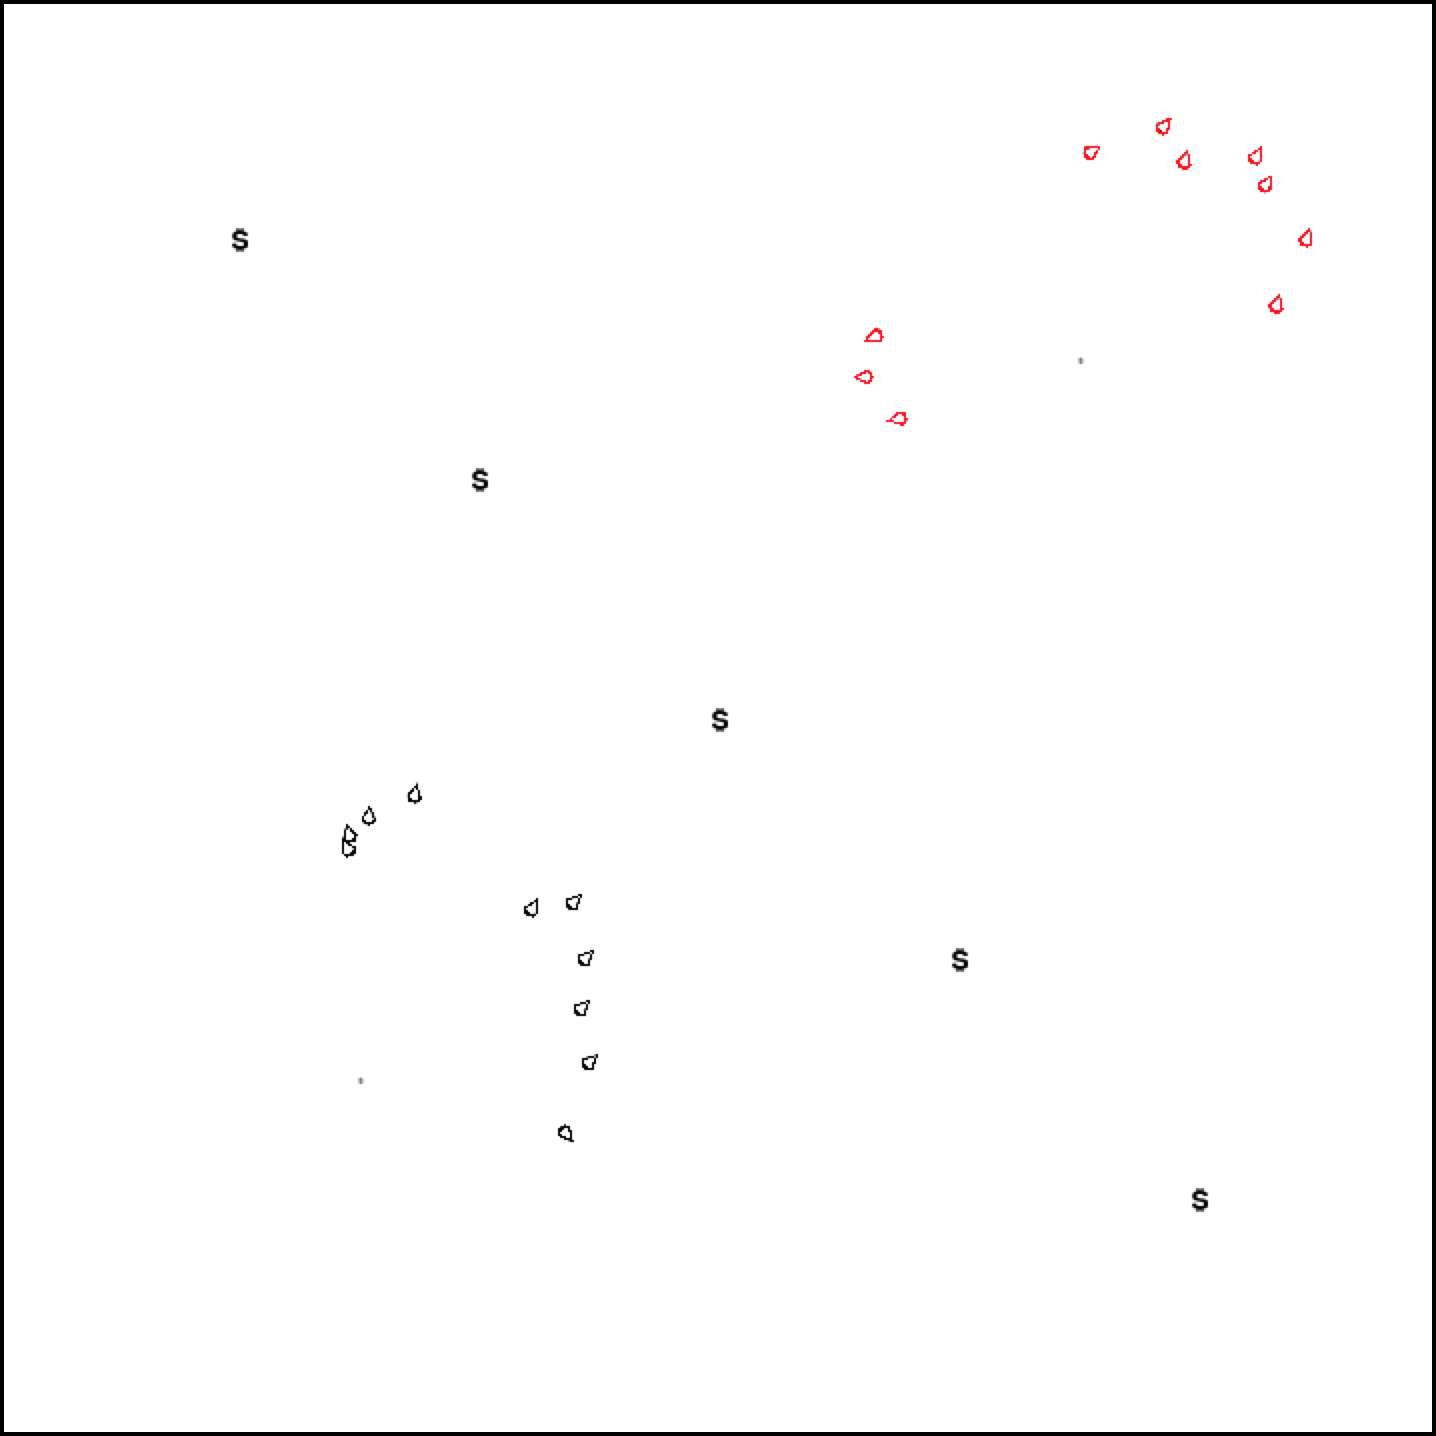
\includegraphics[width=0.5\textwidth]{figures/simulation}
    \caption{Simulation of agents spreading in flocks.}
\end{figure}

Each simulation was run in parallel as subprocess of a master evolutionary computation process. The master process randomly initialized a population of 50 black team configurations, then ran a simulation for each individual in the population. After all 50 simulations were completed, tournament based selection with tournaments of size three were carried over to the next generation along with the 5 most elite individuals. After selection, genetic operators were applied.

In our first experiment we only used mutation to change the states in the finite state machine of the particles. In the second experiment we used recombination in addition to mutation operations. In either case, elite individuals were exempt from genetic operations, however elite individuals could be recombined to replace other individuals in the population. Both the mutation and recombination (when used) had a likelihood of 0.2. Maximum and minimum parameters were also placed on the values of the weight, the radii, and the alpha values to ensure an economic and reasonable result.

\section{Results}
results

\section{Discussion}
This work described herein represents only the first steps in the application of evolutionary techniques to this problem domain. By mutating and applying selective pressure to the movement component parameters, we were able to show that a machine could optimize the parameters better than a person. This was a form of optimization, but it did not result in novel behaviors. Indeed, since we hard-wired the transitions between the states (allowing for the guarding threshold to evolve) and allowed the evolver to mutate existing movement components in a given state but not to add them (i.e., we pre-defined which components could have non-zero weight for each state), we held constant the "meaning" of each state.

The next step would be to evolve the structure of the FSM itself; not only to allow the evolver to mix-in any component to any state, but to allow it to add new states, delete old states, and change the transitions between the states.

\bibliographystyle{plain}
\bibliography{paper}

\end{document}
